

\documentclass{../JAC2003}  % A4
%\documentclass[acus]{JAC2003} % US

\usepackage{graphicx}
\usepackage{booktabs}
\usepackage{color}
\usepackage{multirow}
\usepackage{multicol}
\usepackage[table]{xcolor}
\usepackage{colortbl}
\usepackage{array}

\setlength{\titleblockheight}{27mm}

\hyphenation{op-tical net-works semi-conduc-tor}



%\newcommand \modified[1]{{\textcolor{red}{#1}}}
\newcommand \modified[1]{{\textcolor{black}{#1}}}

\begin{document}

\title{RELIABILITY IN A WHITE RABBIT NETWORK}

% author names and affiliations
% use a multiple column layout for up to three different
% affiliations

\author{

%\IEEEauthorblockN{Bunch of Freaks}
%\IEEEauthorblockA{CERN\\
%Geneva\\
%Email: white.rabbit@cern.ch}

\IEEEauthorblockN{Maciej Lipi\'{n}ski, Tomasz W\l{}ostowski, Javier Serrano, Pablo Alvarez}
\IEEEauthorblockA{CERN, Geneva\\
Email: \{maciej.lipinski, tomasz.wlostowski, javier.serrano, pablo.alvarez.sanchez\}@cern.ch}

}

% conference papers do not typically use \thanks and this command
% is locked out in conference mode. If really needed, such as for
% the acknowledgment of grants, issue a \IEEEoverridecommandlockouts
% after \documentclass

% for over three affiliations, or if they all won't fit within the width
% of the page, use this alternative format:
% 
%\author{\IEEEauthorblockN{Michael Shell\IEEEauthorrefmark{1},
%Homer Simpson\IEEEauthorrefmark{2},
%James Kirk\IEEEauthorrefmark{3}, 
%Montgomery Scott\IEEEauthorrefmark{3} and
%Eldon Tyrell\IEEEauthorrefmark{4}}
%\IEEEauthorblockA{\IEEEauthorrefmark{1}School of Electrical and Computer
%Engineering\\
%Georgia Institute of Technology,
%Atlanta, Georgia 30332--0250\\ Email: see
%http://www.michaelshell.org/contact.html}
%\IEEEauthorblockA{\IEEEauthorrefmark{2}Twentieth Century Fox, Springfield,
%USA\\
%Email: homer@thesimpsons.com}
%\IEEEauthorblockA{\IEEEauthorrefmark{3}Starfleet Academy, San Francisco,
%California 96678-2391\\
%Telephone: (800) 555--1212, Fax: (888) 555--1212}
%\IEEEauthorblockA{\IEEEauthorrefmark{4}Tyrell Inc., 123 Replicant Street, Los
%Angeles, California 90210--4321}}


\maketitle

\begin{abstract}

White Rabbit (WR) is a time-deterministic, low-latency Ethernet-based network which enables 
transparent, sub-ns accuracy timing distribution. It is being developed to replace 
the General Machine Timing (GMT) 
%\cite{biblio:GMT} 
system currently used at CERN and will become 
the foundation for the control system of the Facility for Antiproton and Ion Research (FAIR) 
at GSI. High reliability is an important issue in WR's design, 
since unavailability of the accelerator's 
control system will directly translate into expensive downtime of the machine. 
A typical WR network is required to lose not more than a single message per year. 
Due to WR's complexity, the translation of this real-world-requirement into 
a reliability-requirement constitutes an interesting issue on its own -- a WR network 
is considered functional only if it provides all its services to all its clients at any time. 
This paper defines reliability in WR and describes how it was addressed by dividing it into 
sub-domains: deterministic packet delivery, data 
%redundancy, 
resilience, 
topology redundancy and clock 
resilience. The studies show that the Mean Time Between Failure (MTBF) of the WR Network 
is the main factor affecting its reliability. Therefore, probability calculations for 
different topologies were performed using the "Fault Tree analysis" and analytic estimations. 
Results of the study show that the requirements of WR are demanding. Design changes might be needed 
and further in-depth studies required, e.g. Monte Carlo simulations. Therefore, a direction 
for further investigations is proposed.
\end{abstract}


\section{Introduction}

White Rabbit (WR, \cite{biblio:whiteRabbit}) is a project which aims at creating an
Ethernet-based network with low-latency, deterministic packet delivery
and network-wide, transparent, high-accuracy timing distribution. The
White Rabbit Network (WRN) is based on existing standards, namely
Ethernet (IEEE 802.3 \cite{biblio:IEEE8023}), Synchronous Ethernet
(SyncE \cite{biblio:SynchE}) and PTP \cite{biblio:IEEE1588}. 
It is fully compatible with these standards.

A WRN consists of White Rabbit Nodes (nodes) and White Rabbit Switches
(switches) interconnected by fiber or copper links. 
\modified{The focus of this article is on 1000Base-LX \cite{biblio:IEEE1588} 
single-mode fiber connections only. WR }%It also
supports integration of nodes and/or switches that are not White Rabbit. 
A simple WRN is presented in \figurename~\ref{fig:WRnetwork}.

A node is considered the source and destination of information sent
over the WRN. The information distributed over a WRN includes:
\begin{itemize}
   \item  Timing - frequency and International Atomic Time (TAI).
   \item  Data  - Ethernet traffic between nodes.
\end{itemize} 

In order to understand the goals of the WR project -- namely
determinism, high reliability and accurate synchronization -- these
terms are explained below.

\textbf{Determinism} is guaranteed by having a worst-case upper bound
in frame delivery latency.  

\textbf{Accuracy} is a measure of the deviation between the clock of
the \textit{grandmaster} node\modified{/switch} of a WRN and that of any other node.
Assuming only fiber interconnections, a WRN is meant to achieve
sub-nanosecond accuracy. 

\textbf{Reliability} of a WRN refers to robust delivery of data and
timing to all the nodes.
% data being delivered in a deterministic manner. 
%A WRN is considered reliable only if all the nodes, receive
%data and timing. 
The timing must allow all the nodes to be
synchronized with the required accuracy and the data must always be
delivered on time.
\begin{figure}[!t]
\centering
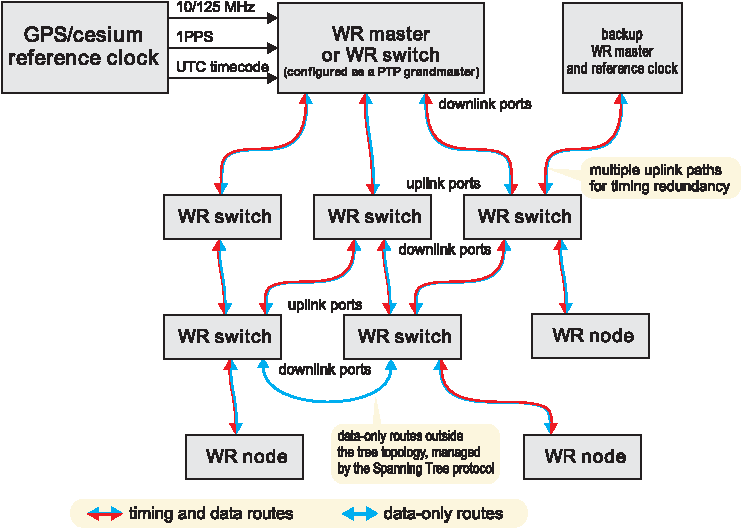
\includegraphics[height=2.10in]{../../figures/network/hierarchy.eps}
\caption{A White Rabbit Network \cite{biblio:TomekMSc}.}
\label{fig:WRnetwork}
\end{figure}

All these features are required to create a timing and control system which may
replace the General Machine Timing (GMT) \cite{biblio:GMT} at CERN and
fulfill a similar role at the Facility for Antiproton and Ion
Research (FAIR) in GSI \cite{biblio:FAIRtimingSystem}. Such system requires 
synchronization of up to 2000 nodes with sub-nanosecond accuracy, 
an upper bound in frame delivery and a very low data loss rate.
However, many other applications of White Rabbit are possible. This includes industry,
telecommunications and other large distributed systems (e.g. distributed
oscilloscopes \cite{biblio:distOscilloscope}).

This article focuses solely on the PTP-based timing distribution in a WRN. PTP is a packet-based
protocol designed to synchronize devices in distributed systems. The accuracy of the PTP
synchronization is implementation-dependent. The standard is foreseen for 
% this is how I understand the fact that corretionField can carry fractional
% nanoseconds and the syncEventEgressTimestamp includes this figures (see e.g.: 
% clause 9.5.9.3, page 103 of PTP
sub-nanosecond accuracies. However, such performance is not achieved in typical PTP
implementations for two reasons:
\begin{itemize}
  \item Limited precision and resolution of PTP timestamps.
  \item Unknown physical link asymmetry. 
\end{itemize}
Additionally, the quality of PTP-syntonization depends on the exchange rate 
of PTP messages. The higher the quality of the clock we want to recover, 
the higher the bandwidth needed for PTP-related traffic.

The precision of timestamps is greatly increased in the existing PTP implementations
by hardware-based timestamping. However, such implementations
are limited by the resolution which is specified by the hardware-driving frequency
(e.g. 8ns for 125MHz).

The asymmetry is not detectable by PTP; if known, PTP corrects for it to increase
synchronization accuracy. Some of the sources of the physical layer asymmetry can be
eliminated by proper network configuration, e.g. excluding routers or non-PTP bridges from the
network. Others, in particular the inaccuracy caused by physical medium asymmetry (i.e.
difference in propagation velocity in two-way communication over fiber) or PCB layout (i.e.
connection length between PHY and timestamping hardware) need to be obtained through proper a
priori-measurement. 

White Rabbit addresses these limitations to achieve sub-nanosecond accuracy
of synchronization. It uses SyncE to distribute the common notion of frequency in the entire
network over the physical medium. It casts the problem of timestamping into a phase detection
measurement. The results of these precise measurements are used both during normal PTP operation
and for quantifying physical medium asymmetry during the calibration phase.
% Consequently, high precision
% timestamps are obtained. Moreover, the parameters necessary to calculate the physical medium
% asymmetry can be determined. 
%This knowledge is used in the PTP computations of the clock offset and link delay. 
The improved performance of the synchronization is accomplished without increasing PTP-related
traffic (it can be actually decreased) since PTP is only governing the synchronization, while the
syntonization is done by SyncE.

A great effort has been made to align WR-specific solutions with the PTP standard and stay fully
compatible with PTP gear. Consequently, WR can be seen as an extension to PTP. This extension,
called WRPTP, defines its own PTP profile and describes all the WR-specific mechanisms which need
to be implemented by a node/switch to enable sub-nanosecond synchronization with another 
nodes/switches. 
\modified{The compatibility with PTP makes WR more likely to be used in existing PTP-based 
systems by gradual and/or partial upgrade to WRPTP. It also enables the creation of hybrid, 
thus cost-effective, systems.}
WRPTP is presented in section~\ref{sec:wrptp} \textit{White Rabbit PTP}.
Section~\ref{sec:hwSupport} presents an example implementation of 
hardware which supports WRPTP. Finally, the measurements of WRPTP performance and conclusions are
presented in the last two sections of this article.

In PTP nomenclature, the main component of a WRN, the switch, is a boundary clock (BC) -- a clock 
that has multiple PTP ports. Similarly, the node is an ordinary clock (OC) --
a clock that has a single PTP port. Consequently, the WRN
can be seen as a set of independently synchronized Master-to-Slave
(M-to-S) links with ports of OC or BC on both sides
(\figurename~\ref{fig:WRnetwork}, red-blue arrows). The ability to
synchronize a single link scales into the ability to synchronize the
entire network. Therefore, in this article, only a single M-to-S link is
considered, where appropriate.




\section{Definition of reliability in a WRN}

A WRN, consisting of White Rabbit Switches (switches) connected by fiber 
or copper, is meant to transport information among White Rabbit Nodes (nodes). We distinguish 
two types of information distributed over the WRN: 
%(1) {\bf Timing} (frequency and International Atomic Time) and 
(1) {\it Timing} (frequency and Coordinated Universal Time) and 
(2) {\it Data} (the Ethernet traffic).
This translates into two types of services provided by the WRN which have their own requirements and
can be handled separately. The requirements are defined by GSI and CERN as the prospective 
users of WR to control their accelerators.


\subsection{Timing Distribution}

Timing is distributed in the WRN from a switch/node called Timing Master (TM) 
to all the other nodes/switches in the network. 
% The TM is usually connected 
% to the external source, such as Global Positioning System (GPS) receiver. 
All the devices in the 
WRN lock their frequency (syntonize) and adjust their local clocks (synchronize) to that of the TM. 
The deviation between the clock of the TM and that of any other node/switch is called {\bf accuracy}. 
A stable and continuous synchronization of all the nodes with an appropriate accuracy is the key 
requirement of the Timing Distribution in the WRN.

\subsection{Data Distribution}

The critical data distributed over the WRN is the one carrying sets of commands (events) which are 
organized into Control Messages (CM). The CMs are sent by a privileged node (Data Master, DM) in the 
payload of the Ethernet frame(s). Therefore, the Data Distribution in the WRN is broken into 
(1) {\it Control Data (CD)}  -- the Ethernet frames carrying CMs, critical, and 
(2) {\it Standard Data (SD)} -- the Ethernet frames which do not carry CMs, non-critical.
The reliability of the WRN depends on the successful delivery of the CD to all 
the designated nodes. The CMs are always broadcast within a VLAN
% \cite{bilbio:vlan}
, which can span 
the entire network. The worst-case upper bound of their delivery latency from the DM to any node in 
the network, regardless of it's location ({\bf maximum distance from the DM}), is required to be 
guaranteed by the network -- this is {\bf a determinism} requirement. 

\subsection{Reliability of the WRN}

The reliability of the WRN relies on the {\bf deterministic} delivery of the CD 
to all the designated nodes and their sufficiently {\bf accurate and stable synchronization}.  
This means that the WRN is considered non-functional if one or more of the following occur:
\begin{Itemize}
  \item A node is synchronized with insufficient accuracy.
  \item A designated node receives corrupted CD or no CD.
  \item The upper-bound delivery latency has been exceeded.
\end{Itemize}
% (1) A node is synchronized with insufficient accuracy;
% (2) A designated node receives corrupted CD or no CD;
% (3) The upper-bound delivery latency has been exceeded.
Unreliability is translated into the number of CMs considered lost (not delivered, delivered 
corrupted or in a non-deterministic way) in a given period of time. During this time,  
the synchronization must be always of the required quality. 
Quantitative requirements of the accelerator facilities are listed in Table~\ref{tab:requirements}.

\begin{table}[ht]
\caption{GSI's and CERN's requirements summary.} 
\centering
	\begin{tabular}{| l | c | c |}                        \hline
%\textbf{Requirement}& \multicolumn{2}{|c|}{\textbf{Value(s)}}     \\
\rowcolor{gray!35}{}
\textbf{Requirement}     & {\bf GSI}        & {\bf CERN}          \\ \hline
Max latency    		 & 100$\mu s$       & 1000$\mu s$         \\ \hline
CM failure rate          & $3.17*10^{-12}$  & $3.17*10^{-11}$     \\ \hline
CMs lost per year        & 1                & 1                   \\ \hline
$d_{max}$ from DM        & 2km              & 10km                \\ \hline
CM size 		 & 200-500 bytes    & 1200-5000 bytes     \\ \hline
Accuracy	  	 & probably 8ns     & 1$\mu s$ to  ~2ns   \\
%accuracy                 &                  & few nodes  ~2ns     \\
\hline

\end{tabular}
\label{tab:requirements}
\end{table}

\section{Failure Study}

One of the main possible reasons for WRN failure, which affects both Timing and Data Distribution, is 
a malfunction of its elements (switches or links). Since the distribution of information 
in the WRN is of one-to-all character (Data/Timing Master to all nodes), all the elements of the WRN are 
considered Single Points of Failure (SPoF)\cite{biblio:mtbf}. Malfunction of any SPoF 
results in failure of the entire system.
SPoFs can be eliminated by introducing redundancy of the system components. Due to its special features 
(distribution of frequency over physical layer) and strict requirements (determinism, low data loss), 
the number of possible redundant topologies of the WRN is restricted, as explained in the 
following sections. 

Imperfections of the physical medium as well as switching between redundant elements of the network 
(which takes time) can cause loss or corruption of data. The deterministic and \modified{mostly} broadcast character 
of the data distribution in the WRN enforces application of the Forward Error Correction (FEC) 
%\cite{biblio:coding} 
-- adding redundant information on transmission to enable recovery of lost or corrupted data 
on reception. This brings constant data overhead and the probability that the added redundancy is 
not sufficient to recover the data. However, it is the price to pay for ensuring low latency 
and determinism of data delivery in the WRN. 

The delivery latency of an Ethernet frame varies with cable length and the number of hops (switches) 
it has to traverse to reach its destination, the traffic load on the way and 
the assigned Class of Service (CoS). Therefore, to ensure the required determinism 
of the CD delivery, we need to make sure that there is no congestion of Ethernet frames 
carrying CMs. Moreover, the number of hops (the latency introduced by them) needs to be 
sufficiently small, which can be done by restricting the topology. 

The resilience of the Clock Distribution translates into continuous and stable 
synchronization of all the nodes and switches in the WRN (Table~\ref{tab:requirements}). Although, 
the network redundancy eliminates SPoFs, the switch-over between redundant elements might introduce 
instability and render the network unreliable despite the costly redundancy. 
Therefore, a seamless switch-over between redundant clock paths needs to be ensured. 
Another reason for the deterioration of the synchronization 
accuracy is the variation of external conditions (e.g. temperature) which needs to be compensated.

% In terms of the Data Distribution reliability, the topology redundancy can turn out to be 
% useless, if the switch-over between redundant elements causes more data to be lost then the 
% capabilities of FEC scheme.
% {\it [add here, change the rest]}
% In summary, we need investigate how to :
% \begin{Itemize}
%   \item  eliminate/decrease data loss due to :
%     \begin{Itemize}
%       \item physical medium imperfection,
%       \item switch over between redundant elements,
%       \item traffic congestion,
%     \end{Itemize}
%   \item eliminate synchronization instability due to:
%     \begin{Itemize}
%       \item switch over between redundant data paths,
%       \item external condition variations,
%       \item Ethernet frame loss (PTP),
%     \end{Itemize}
%   \item ensure required upper-bound delivery latency of Control Data.
% \end{Itemize}


\section{Determinism}

% The delivery latency of an Ethernet frame varies with cable length and the number of hops (switches) 
% it has to traverse to reach its destination, the traffic load on the way and 
% the assigned Class of Service (CoS, \cite{bilbio:vlan}). 
A carefully configured and properly used WRN offers deterministic Ethernet frame delivery 
thanks to the implementation of CoS and the fact that the delay introduced by the switch can be 
verified by analysis of {\bf publicly available source code} \cite{biblio:whiteRabbit}. 
Such analyses were performed to verify the worst-case upper bound 
delivery latency of a CM against the requirements listed in the Table~\ref{tab:requirements}. 
The results, presented in Table~\ref{tab:CMlatency} ({\it Store-and-forward} column), 
take into account the fact that a CM is encoded into 4 Ethernet frames (as required by the FEC 
and described in the next Section), it is sent with the highest priority (CoS) and it always 
traverses 3 hops.

\begin{table}[ht]
\caption{Control Message(CM) deliver latency estimations.} 
\centering

	\begin{tabular}{| c | c | c | c | c | c |}          \hline
\rowcolor{gray!35}{}
               & \multicolumn{4}{|>{\columncolor{gray!35}}c|}{\textbf{CM deliver latency}}                    \\ \cline{2-5}
\rowcolor{gray!35}{}
\textbf{CM size}& \multicolumn{2}{|>{\columncolor{gray!35}}c|}{\textbf{Store-and-forward}} 
                &\multicolumn{2}{|>{\columncolor{gray!35}}c|}{\textbf{Cut-through}}                           \\\cline{2-5}
\multicolumn{1}{|>{\columncolor{gray!35}}c|}{} &
\multicolumn{1}{|>{\columncolor{gray!35}}c|}{GSI} &
\multicolumn{1}{|>{\columncolor{gray!35}}c|}{CERN} &
\multicolumn{1}{|>{\columncolor{gray!35}}c|}{GSI} &
\multicolumn{1}{|>{\columncolor{gray!35}}c|}{CERN} \\ \hline
%		&    GSI           & CERN          &    GSI           & CERN          \\ \hline
%200 bytes      & ???$\mu s$       & ???$\mu s$    & ??$\mu s$        & ???$\mu s$    \\ \hline
500 bytes      & 221$\mu s$       & 283$\mu s$    & 76$\mu s$        & 118$\mu s$    \\ \hline
1500 bytes     & 285$\mu s$       & 325$\mu s$    & 102$\mu s$       & 142$\mu s$    \\ \hline
5000 bytes     & 324$\mu s$       & 364$\mu s$    & 162$\mu s$       & 202$\mu s$    \\ \hline
\end{tabular}
\label{tab:CMlatency}
\end{table}

The analysis revealed that GSI's requirements are not fulfilled: the upper-bound delivery latency
for the required size of CM and max distance of 2km is greater then 100$\mu s$. 

The solution to decrease delivery latency is targeted into the CD only and 
takes advantage of its characteristics (broadcast within a VLAN, sent by privileged node). 
We propose to break the highest priority of 
the CoS into two (unicast and broadcast) and use the highest priority broadcast Ethernet traffic only for 
the CD. Moreover, this particular traffic shall be forwarded using the cut-through method 
(unlike the store-and-forward method used normally in the switch) which can be effectively fast 
for the broadcast traffic with a single source (DM). The results, 
presented in Table~\ref{tab:CMlatency} ({\it Cut-through} column), show a significant improvement. 
The solution requires hardware-supported cut-through forwarding in the switch as described 
in \cite{biblio:robustness}. 



\section{Data Resilience}


\subsection{Forward Error Correction}
\label{sec:fec}

The objective of the FEC scheme is to decrease the loss rate of the CMs, preferably, 
to less then one per year. WR uses as a physical medium Fiber Optic and CAT-5. The number 
of received corrupted bits compared to the total number of received bits is called Bit Error Rate 
(BER). The value of BER  characterizes a physical medium and can be used to characterize the entire 
switched network.
%  if the following factors are taken into account: 
% (1) {\it type of cabling} (fiber/twisted pair),
% (2) {\it logic topology},
% (3) {\it network address} (broadcast/unicast).
A WRN can be seen as a Packet Erasure Channel (PEC) or as a Binary Erasure Channel (BEC) depending 
on the effect of a bit error on the frame. If the frame is lost (e.g. dropped by the switch due to 
a corrupted header or lost during switch-over between redundant components), the WRN is a PEC. 
If the bit error happens in the link between a switch and node, a corrupted frame 
\modified{can be used (optional)}
%is used 
to attempt frame recovery. In such case, the channel is called BEC. Each type of channel requires 
a different FEC solution. Therefore two concatenated FECs are used in WR. 
Reed-Solomon (R-S) %\cite{biblio:r-s} 
%\cite{biblio:coding} 
coding is used for the PEC and 
allows to encode k original-frames into n encoded-frames ($n>k$). 
Reception of any k encoded-frames can be used to decode the original frames. 
\modified{Hamming coding with additional parity (SEC-DED)} 
%Hamming coding 
is used for the BEC and allows to detect up to two simultaneous bit errors and 
correct a single error.
These two schemes (R-S and Hamming) are combined to encode each CM -- it is 
split into two and encoded using R-S into four messages (two original and two 
with redundant data). Each of the four messages is then encoded using Hamming. Such encoded 
messages are sent in a burst of 4 Ethernet frames. Reception of any two of these frames enables 
to decode the original Control Messages. 
A systematic analysis, using the BER characteristic of the WRN, proves that the presented FEC scheme 
guarantees less than single CM lost per year due to physical medium 
imperfection, as can be seen from Table~\ref{tab:gsi_cern_fec}. 

\begin{table}[ht]
 	\begin{center}
\caption{GSI and CERN FEC characteristics.}
\begin{tabular}{|p{4cm}|c|c|} \hline
%	\cline{2-3}
%	&  \multicolumn{2}{|c|}{Use Case} \\ \cline{2-3}
\rowcolor{gray!35}{}
{\bf Parameter}	&  {\bf GSI} & {\bf CERN} \\ \hline
	\multicolumn{1}{|p{4cm}|}{Control Message length} & 500 bytes & 1500 bytes     \\ \hline
	\multicolumn{1}{|p{4cm}|}{Control Message per year} & $3.145 10^{11} $ &$  3.145 10^{8} $ \\ \hline
	\multicolumn{1}{|p{4cm}|}{Max Bit Correct.} & 1 & 1  \\ \hline
%	\multicolumn{1}{|p{4cm}|}{Parity-Check Bits} & 13    &  13   \\ \hline
%	\multicolumn{1}{|p{4cm}|}{PEC Code Overhead} & 3  & 2 \\ \hline
%	\multicolumn{1}{|p{4cm}|}{Payload Length} & 400 b  & 800b \\ \hline
	\multicolumn{1}{|p{4cm}|}{Payload Length} & \modified{294 bytes}  & \modified{854 bytes} \\ \hline
	\multicolumn{1}{|p{4cm}|}{Num Encoded Frames} & 4  & 4 \\ \hline
	\multicolumn{1}{|p{4cm}|}{Needed Frames to Receiver} & 2 & 2 \\ \hline
	\multicolumn{1}{|p{4cm}|}{Probability of Loosing a CM} & $10^{-14}$ & $10^{-13}$\\ \hline
	\end{tabular}   
	
	\label{tab:gsi_cern_fec}
	\end{center}
\end{table}

\subsection{Rapid Spanning Tree Protocol (RSTP)}

In an Ethernet network with redundant topology, the problem of loops (causing "broadcast storms") 
is handled by the Rapid Spanning Tree Protocol (RSTP)
% \cite{biblio:IEEE8021D}
. It creates a loop-free 
logical topology by blocking appropriate ports in switches, and unblocks them in case of topology 
break (due to element failure).

The functionality provided by the RSTP is essential for the WRN. However, the convergence speed 
provided by the standard implementation of the RSTP (milliseconds 
%\cite{biblio:RSTPperf} 
at best) 
would cause many CMs to be lost during the process. This is not acceptable, we need 
a solution which is fast enough to prevent loosing the CMs at all. Since we know the 
size-range of the CMs (Table~\ref{tab:requirements}) and how they are FEC-encoded into Ethernet frames,
we can calculate the maximum value of the convergence time: 3$\mu s$. This time is smaller than 
the duration of transmitting a single frame with FEC-encoded CM -- this ensures that no more than 
two frames with FEC-encoded CM are lost, thus the CM can be recovered.

In order to achieve a convergence time of 3$\mu s$, the switch-over between active 
and backup connections needs to be performed in the hardware as soon as the link-down is detected. 
It can only be done if the alternative topology is known in advance. The knowledge of alternative 
topology is translated into an RSTP-assignment of alternative and backup roles of switch ports, 
i.e at least one port with alternative role must be identified in every switch 
(except the topology-root switch).    
%\modified{, i.e at least one port with each of these roles must be identified in every switch}.
%
%If at least one port of a switch is assigned an alternative role, it means that 
%the RSTP algorithm establishes more than one path to the topology-root switch and therefore 
%the alternative topology is know in advance. 
%Such ports are identified when the RSTP algorithm establishes more than one path to the 
%topology-root switch and all paths can be used simultaneously, 
%
If we ensure, by restricting the topology, that RSTP identifies the alternative links, 
we can use its data to feed the hardware, consequently achieving the required convergence time 
and staying standard-compatible: 
the hardware switch-over is just a faster RSTP-driven convergence. The required topology 
restrictions, described in \cite{biblio:robustness}, greatly overlap with these imposed by 
the Time Distribution. 

 



\section{Clock Distribution}


% The resilience of the Clock Distribution translates into continuous and stable 
% synchronization of all the nodes and switches in the WRN (Table~\ref{tab:requirements}).
% A loss of time notion in a node can be caused by a link or switch failure - break of clock path 
% between the TM and the node. In order to prevent synchronization break, redundancy of network 
% elements (switches, cables) can be introduced ensuring redundant clock paths. However, 
% the switch-over between redundant elements might introduce instability and render the network 
% unreliable despite the costly redundancy. Therefore, the seamless switch-over between redundant 
% clock paths is one of the design-goals to enable network topology redundancy and, as a consequence, 
% offer robust and stable synchronization. The other reasons for the deterioration of synchronization 
% accuracy are the variation of external conditions (e.g. temperature) and loss of Ethernet frames with 
% timing information (PTP).  

%\subsection{Switch-over}

A seamless switch-over between redundant sources of timing (uplink ports) is heavily supported by 
the Clock Recovery System (CRS) \cite{biblio:TomekMSc} of the switch and the WR extension to PTP 
(WRPTP)\cite{biblio:WRPTP}. 

Figure~\ref{fig:switch-over} presents an example where a switch (timing slave) is connected 
(by its uplinks 1 \& 2) 
to two other switches (primary and secondary masters) -- the sources of timing. On both 
uplinks the frequency is recovered from the signal and provided to the CRS. Similarly, WRPTP 
measures delay and offset on each of the links and provides this data to the CRS. 
The modified Best Master Clock (mBMC) algorithm \cite{biblio:WRPTP} decides which of the 
timing masters is "better" and elects it the primary, the other is considered secondary (backup).
The information from {\it uplink 1} (primary) is used to control 
the CRS and adjust the local time. However, at any time all the necessary information from the 
{\it uplink 2} is available and a seamless switch-over can be performed in case of 
primary master failure \cite{biblio:TomekMSc}.

\begin{figure}[t]
\centering
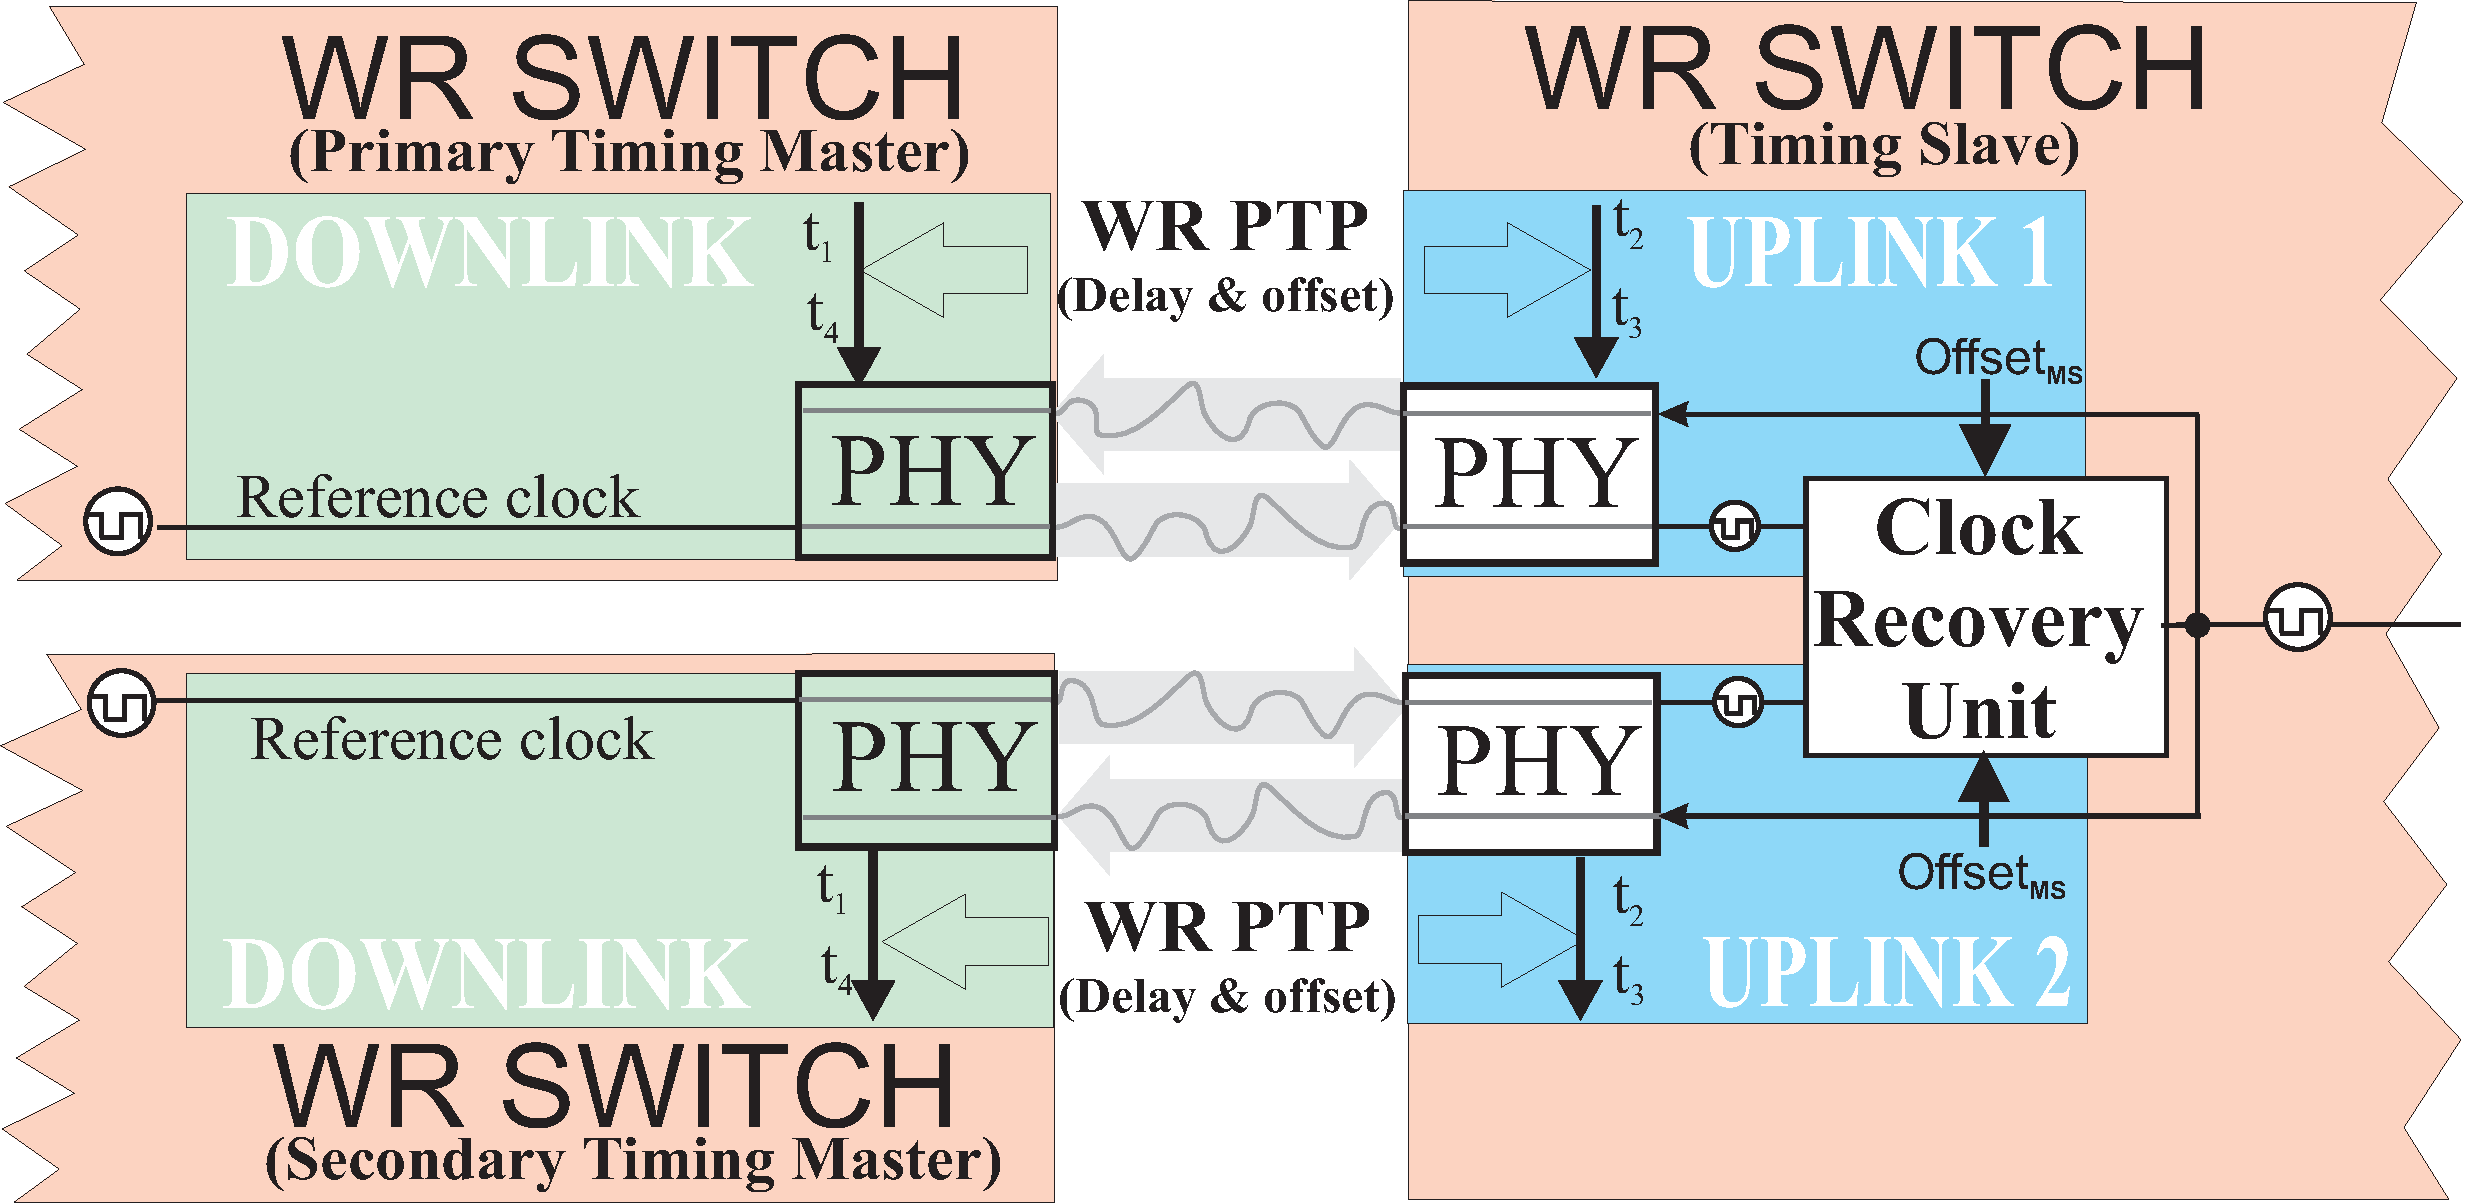
\includegraphics[width=3.2in]{robustness/clockDistribution.pdf}
\caption{Seamless switch-over.}
\label{fig:switch-over}
\end{figure}

%\subsection{Variable conditions and loss of PTP messages}
In addition to the switch-over-related synchronization instability, the variation of external temperature 
can cause an accuracy degradation. This problem, however, is solved by the PTP standard itself. By 
frequent link delay measurements, the fluctuation is compensated. 





\section{Overall Reliability}

The final equation of the WRN reliability is a sum of the data and clock distribution reliabilities.
The clock distribution is assumed to be sufficiently accurate as long as there is a connection 
between the TM and all the nodes. The same applies to the CD distribution: 
as long as there is a valid connection, the FEC makes sure that the data is delivered with 
a sufficient reliability and the latency calculations prove it to be deterministic while the 
congestion is prevented by CoS and limited number of data sources (DM). Consequently, the overall 
reliability is strongly dependent on the WRN topology, which needs to be appropriate for the proposed 
solutions (SyncE, H/W-supported RSTP, upper-bound latency). 

For the comparison of different network topologies, we consider the reliability of a network of 
switches. 
%with M inputs (connected to DM/TM). 
Each node is connected to such a network with M links 
(each to a separate switch). The value of M reflects the level of redundancy 
(M=1 for no redundancy, M=2 for double redundancy, etc).


In the calculations of the network reliability we used the idea of Mean Time Between Failure (MTBF) 
and its relation with the failure probability presented in \cite{biblio:mtbf} 
(a very simplified mathematical model). In order to calculate the MTBF of the entire network, we need the 
MTBFs of each network component: switches and links. Since the WR switches are still under 
development (no MTBF measured), we used representative values for CISCO switches 
({2, 10 and 100}$*10^4$[h]). Two estimation methods were used: "Fault Tree analysis" 
\cite{biblio:faultTree} and analytic. Both provide just rough estimations of the reliability. 
The former allowed to estimate two-terminal reliability (DM to single node) 
%\cite{biblio:INF_TECH} 
of simple non/double/triple-redundancy topologies ($P_f$). The most desired value is the 
all-terminal network reliability ($P_{f\_Network}$), where : $P_f < P_{f\_Network} < N_{nodes}*P_f$. 
Table~\ref{tab:2000nodesReliability} 
presents rough estimations of $P_{f\_Network}$ using analytic calculations for the three considered 
topologies ($MTBF_{Switch}$=200 000[h]). However, to meet the requirement of $\approx$2000 nodes and 
only three network layers (hops), 
\modified{the Data Master node is connected to more separate switches than 
the level of redundancy (M).}
% the topologies are of the type M-inputs/N-outputs, where 
% $N \geq M$.
The estimations show that a triple redundancy topology can barely satisfy the requirements by CERN 
(Table~\ref{tab:requirements}).

% \begin{figure}[t]
% 	 \centering
% 	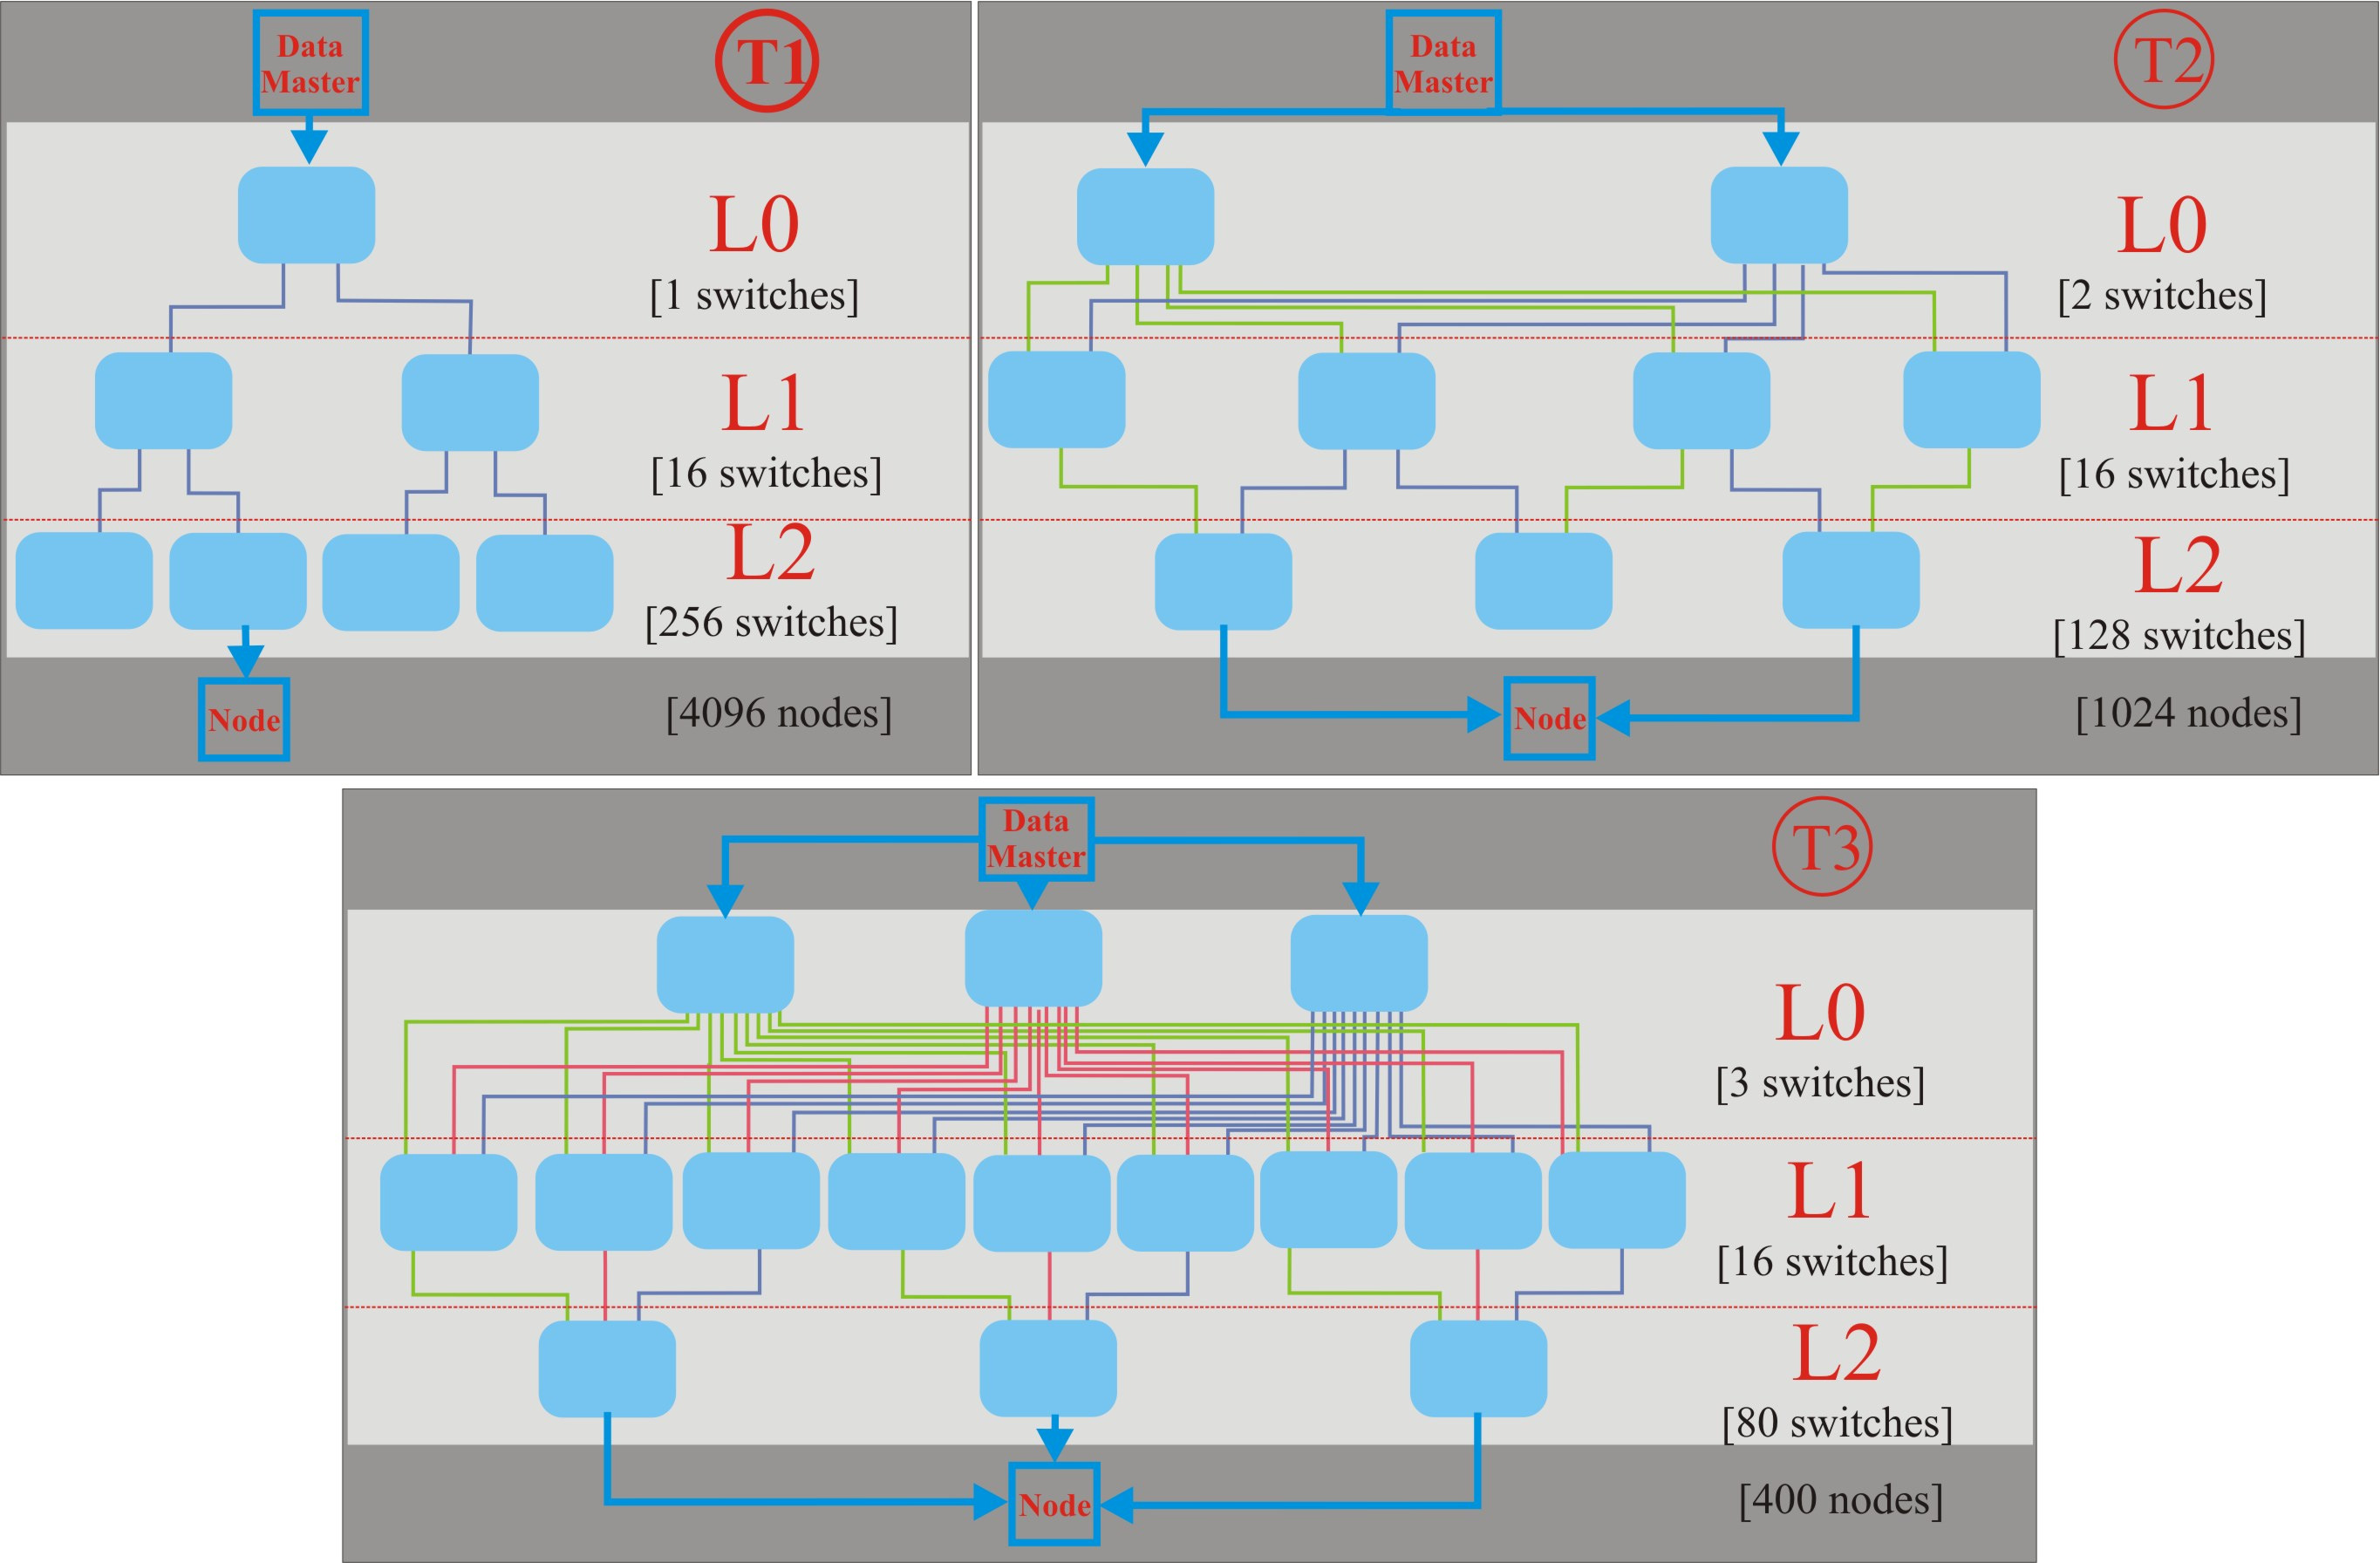
\includegraphics[width=3.4in]{fig/threeTopologies.ps}
% 	\caption{Examples of topologies with different level of redundancy.}
% 	\label{fig:threeTopology}
% \end{figure}

\begin{table}[ht]

%\caption{Different topologies ($\approx 2000$ nodes).}
\caption{WRN topologies's reliabilities.}
\centering
%\rowcolors {0}{gray!35}{}

\begin{tabular}{| c | c | c | c |}        \hline
%{\bf Redundancy}& \textbf{Switches}  & \multicolumn{2}{| c |}{\textbf{$MTBF_{Switch}$=  20 000[h] }} \\
%                &                    & $P_f$                       & MTBF[h]               \\ \hline
\rowcolor{gray!35}{}
{\bf Redundancy}& \textbf{Switches}  & $P_f$                       & MTBF[h]               \\ \hline
No              &  127               & $ 2.08*10^{-3}$             & $ 5.77*10^{3}$        \\ \hline
Double          &  292               & $ 4.71*10^{-7}$             &  $ 2.55*10^{7}$       \\ \hline
Triple          &  495               & $ 3.06*10^{-11}$            &  $ 4.08*10^{11}$      \\ \hline
\end{tabular}
\label{tab:2000nodesReliability}
\end{table}



\section{Conclusions}
\label{sec:conclusions}

In this paper the first deployment of a ``beta version" of a White Rabbit
system is described. The deployed system includes a WR Network (consisting of switches) 
interconnecting WR Nodes. 

The results indicate that a system based on the 
White Rabbit technology is capable of providing nanosecond accuracy of synchronization 
over large distances (i.e. over 16 km). The measured accuracy of the deployed system  
is 0.517~ns and the precision is 0.119~ns. The calculated MTIE is below 1.05~ns
with only 0.0003$\%$ of values exceeding the $\pm$0.5~ns range.
The WR-timebase 
guarantees sub-nanosecond accuracy and tens of picoseconds precision of the distributed time 
and frequency reference regardless of the changing temperature conditions. 
The standard deviation of the skew measured between the time reference (grandmaster) and 
the nodes (over a peak-to-peak 45 
degrees Celsius temperature range) is 55~ps while the MTIE is below 342~ps. 
The temperature tests indicate that the acceptable influence   
of the temperature variation of WR devices on the quality of synchronization can be easily
reduced by compensating temperature-induced changes of the hardware delays. 
Such a compensation should be considered in future developments of the WR technology.

The high accuracy and precision time transfer over an Ethernet-based WR Network has many potential
applications. Precise time-tagging of the input events using WR-provided timebase is the first to
be realized. Therefore, the described deployment marks an important milestone in the White Rabbit Project -- 
proof-of-concept technology becomes a working solution. This solution is about to be 
commercially available while sustaining its openness (open hardware and open software). 


\newpage



\bibliographystyle{IEEEtran}
\bibliography{IEEEabrv,./biblio}

\end{document}


